
%%%%%%%%%%%%%%%%%%%%%%%%%%%%%%%%%%%%%%%%%%%%%%%%%%%%%%%%%%%%%%%%%%%%%%%
%%%%%%%%%%%%%%%%%%%%%%%%%%%%%%%%%%%%%%%%%%%%%%%%%%%%%%%%%%%%%%%%%%%%%%%
%%%%%%%%%%%%%%%%%%%%%%%%%%%%%%%%%%%%%%%%%%%%%%%%%%%%%%%%%%%%%%%%%%%%%%%
%%%%%%%%%%%%%%%%%%%%%%%%  EJERCICIOS %%%%%%%%%%%%%%%%%%%%%%%%%%%%%%%%%%
%%%%%%%%%%%%%%%%%%%%%%%%%%%%%%%%%%%%%%%%%%%%%%%%%%%%%%%%%%%%%%%%%%%%%%%
%%%%%%%%%%%%%%%%%%%%%%%%%%%%%%%%%%%%%%%%%%%%%%%%%%%%%%%%%%%%%%%%%%%%%%%
%%%%%%%%%%%%%%%%%%%%%%%%%%%%%%%%%%%%%%%%%%%%%%%%%%%%%%%%%%%%%%%%%%%%%%%

\newpage

\section*{Ejercicios}
\addcontentsline{toc}{section}{\textit{Ejercicios}}

%%%%%%%%%%%%%%%%%%%%%%%%%%%%%%%%%%%%%%%%%%%%%%%%%%%%%%%%%%%%%%%%%%%%%%%
%%%%%%%%%%%%%%%%%%%%%%%%% EJERCICIOS 1 %%%%%%%%%%%%%%%%%%%%%%%%%%%%%%%%
%%%%%%%%%%%%%%%%%%%%%%%%%%%%%%%%%%%%%%%%%%%%%%%%%%%%%%%%%%%%%%%%%%%%%%%

\begin{Enunciado}
\subsection*{Ejercicio 1}

Queremos estudiar las características de una unión abrupta PN de silicio a temperatura ambiente con boro (\(10^{15} \, \text{cm}^{-3}\)) y fósforo (\(5,0 \times 10^{14} \, \text{cm}^{-3}\)), siendo la longitud de la zona P de \(0,008 \, \text{cm}\) y la de la zona N de \(0,008 \, \text{cm}\) y el área del contacto de \(10^{-2} \, \text{cm}^2\). 

Las movilidades de electrones y huecos son \(1360 \, \text{cm}^2/(\text{V}\cdot\text{s})\) y \(460 \, \text{cm}^2/(\text{V}\cdot\text{s})\) respectivamente y \(\tau_p = \tau_n = 10^{-6} \, \text{s}\).

\begin{enumerate}[label=\alph*)]
\item En situación de equilibrio, calcula y representa lo siguiente:
\begin{itemize}
    \item La anchura de todas las regiones del dispositivo.
    \item Las bandas de energía incluyendo la banda de conducción, la de valencia, el nivel de Fermi, y el de Fermi intrínseco. Calcula la distancia relativa entre todos esos niveles.
\end{itemize}

\item Si polarizamos la zona N con 0,2 voltios respecto a la zona P, calcula y representa:
\begin{itemize}
    \item La anchura de todas las regiones del dispositivo.
    \item Las bandas de energía incluyendo la banda de conducción, la de valencia, el nivel de Fermi, y el de Fermi intrínseco. Calcula la distancia relativa entre todos esos niveles.
\end{itemize}

\item Si polarizamos la zona N con 0,2 voltios respecto a la zona P, calcula y representa:
\begin{itemize}
    \item El campo eléctrico, densidad de carga y el voltaje en todo el dispositivo.
    \item Las corrientes que surgen a lo largo de todo el dispositivo para cada portador.
\end{itemize}
\end{enumerate}
\end{Enunciado}


Vamos a calcular las masas efectivas en función de las movilidades y las vidas medias:

\begin{equation}
    \mu_n = D_n \frac{q}{kT} = \frac{q}{kT} \tau_n v^2_{th} = \frac{q}{kT} \tau_n \frac{3kT}{m_n^*} = \frac{3q\tau_n}{m_n^*}
\end{equation}
Entonces:
\begin{equation}
    m_n^* = \frac{3q\tau_n}{\mu_n} \qquad m_p^* = \frac{3q\tau_p}{\mu_p^*}
\end{equation}
Usando estas ecuacioens obtenemos:

\begin{equation}
    m_p^* = 3.88 \cdot 10^6 \ m_e \tquad m_n^* = 11.5 \cdot 10^6 \ m_e
\end{equation}
Francamente no se que puede estar mal, pero usaremos las masas típicas $m_p^* = 0.81m_e$ y $m_n=1.18 m_e$. 
\begin{enumerate}[label=\alph*)]
    \item Tenemos que calcular la anchura de todas las regiones del dispositivo y las bandas de energía (banda de conducción, banda de valencia, nivel de Fermi y nivel de Fermi intrínseco). También tenemos que calcular las distancias relativas entre los niveles (lo cual es obvio dado lo anterior). 
    
    Primero tenemos que calcular las distancias, lo cual es simplemente aplicar las fórmulas para la situación de equilibrio
    \begin{equation}
        x_p = \ccorchetes{\frac{2K_S\varepsilon_0}{q} \frac{N_D}{N_A(N_A+N_D)}  V_{bi}}^{1/2}  \qquad 
        x_n = \ccorchetes{\frac{2K_S\varepsilon_0}{q} \frac{N_A}{N_D(N_A+N_D)}  V_{bi}}^{1/2}
    \end{equation}
    Así pues, los valores numéricos son: 

    \begin{equation}
        x_p = 5.000\cdot 10^{-5}  \ [\cm] \qquad x_n =1.000\cdot 10^{-4}  \ [\cm] \qquad W = x_n + x_p = 1.5 \cdot 10^{-4} \ [\cm ]
    \end{equation}
    Y luego tenemos que calcular los valores de todas y cada una de las bandas. Para conocer las banda, teniendo en cuenta que $E_F=0 \ [\eV]$  \textit{a lo largo de todo el dispositivo pn}. Por el resto simplemente aplicar las ecuaciones de la sección 2, tal que en la zona $p$ los valores son los que típicamente esperaríamos para un semiconductor $N_A$, mientras que en la zona $n$ será los que esperaríamos en un conductor $N_A$ menos $V_{bi}$. En la \textit{zona de vaciamiento} los valores de las bandas simplemente valdrán su valor en $p$ menos el valor $V(x)$:
    \begin{equation*}
        V_{bi} = \frac{kT}{q} \ln \parentesis{\frac{N_AN_D}{n_i^2}} = 0.580 \ [\unit{V}]
    \end{equation*}
    \begin{equation*}
        V(x) = \left\lbrace \begin{array}{ll}
            - \frac{qN_A}{2K_S\varepsilon_0} \parentesis{x_p + x}^2  & \ - x_p \leq x \leq 0 \\
            - \frac{qN_D}{2K_S\varepsilon_0} \parentesis{x_n - x}^2 + V_{bi}  & \ 0 \leq x \leq x_n \\
        \end{array} \right.
    \end{equation*}
    Por el resto de situaciones, tenemos que en la zona $p$ las ecuaciones son:
    \begin{equation*}
        E_i = - kT \ln \parentesis{\frac{n}{n_i}} = kT \ln \parentesis{\frac{N_A}{n_i}} \qquad E_c  = E_i  + kT \ln \parentesis{\frac{N_c}{n_i} } \qquad E_v  =E_c-E_g
    \end{equation*}
    tal que 
    \begin{equation*}
        E_g = 1.12 \ [\eV] \qquad N_C = 2 \parentesis{\frac{m_n^* kT}{2\pi \hbar^2}}^{3/2}  = 3.21 \cdot 10^{19} \ [\cm^{-3}] \end{equation*}
    \begin{equation*}    
       N_V = 2 \parentesis{\frac{m_p^* kT}{2\pi \hbar^2}}^{3/2} = 1.83 \cdot 10^{19} \ [\cm^{-3}] 
    \end{equation*}
    \begin{equation*}
        n_i = \sqrt{N_CN_V} e^{-E_g/2kT} = 9.49 \cdot 10^9 \ [\cm^{-3}]
    \end{equation*}
    Así pues obtenemos los siguientes resultados numéricos: 
    \begin{center}
        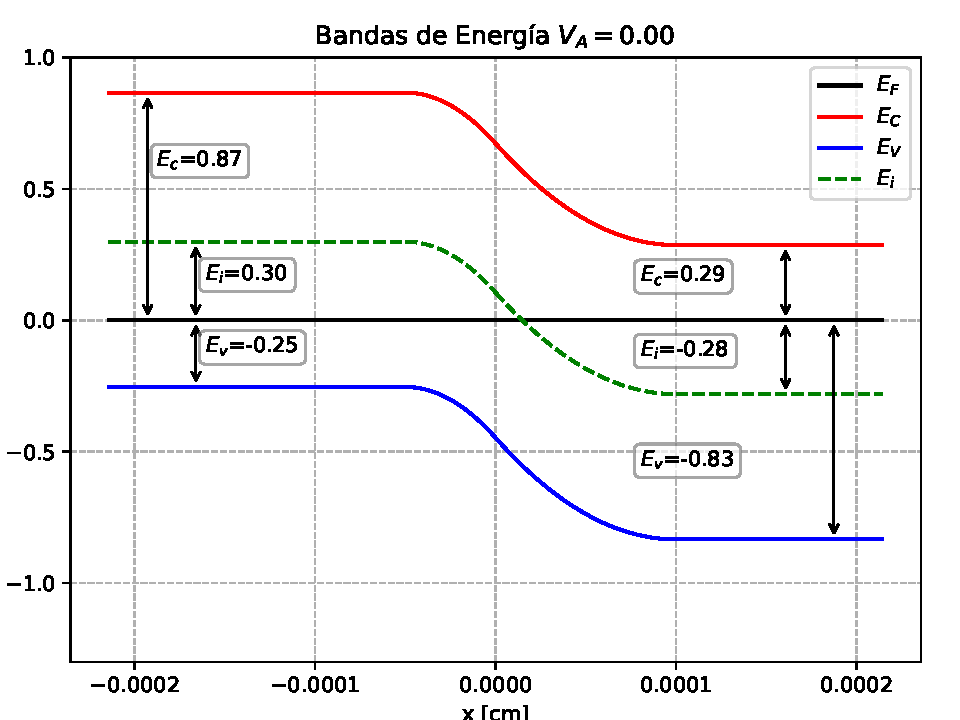
\includegraphics[width=0.85\linewidth]{Ejercicios/Ch_03/03_01_Bandas.pdf}
    \end{center}
    \item Si polarizamos la zona N con 0.2 voltios ($V_A=-0.2$V) estamos en el régimen de polarización inversa. El calculo de los anteriores valores es exáctamente igual solo que ahora tenemos que $V_{bi}\rightarrow V_{bi}-V_A$. Así pues:
    \begin{equation}
        x_p = 5.79867 \cdot 10^{-5}  \ [\cm ] \tquad
        x_n = 1.15973 \cdot 10^{-4}  \ [\cm ]
    \end{equation}
    \begin{center}
        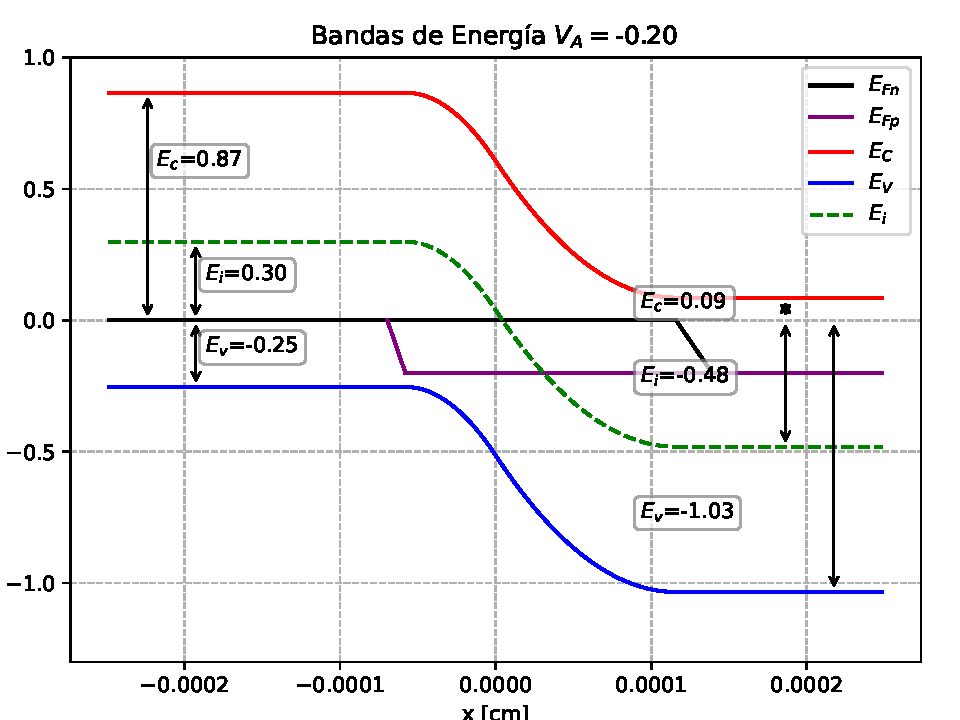
\includegraphics[width=0.7\linewidth]{Ejercicios/Ch_03/03_02_Bandas.pdf}
    \end{center}

    \item Ahora nos piden calcular el campo eléctrico, la densidad de carga y el voltaje a lo largo del dispositivo, así como las corrientes a lo largo del mismo. Para calcular el campo eléctrico tenemos que usar la típica fórmula:

    \begin{equation}
        \Ecal = - \derivadas{V}{x} = \frac{1}{q} \derivadas{E_i}{x}
    \end{equation}
    Así por lo tanto tenemos que: 

    \begin{equation*}
        \Ecal(x) = \left\lbrace \begin{array}{ll}
            - \frac{qN_A}{K_S\varepsilon_0} \parentesis{x_p - x}  & \ - x_p \leq x \leq 0 \\
            - \frac{qN_D}{K_S\varepsilon_0} \parentesis{x_n - x} & \ 0 \leq x \leq x_n \\
        \end{array} \right.
    \end{equation*}
    siendo 0 en el resto de puntos del dispositvo. El volaje se calcula teniendo en cuenta la anterior ecuación (considerando que el cero del potencial está en la zona $p$) on la ecuación que hemos usado previamente (a). Solo falta calcular la densidad de carga, que se hace usando, por ejemplo, la ecuación de Maxwell

    \begin{equation}
        \nabla \cdot E = \frac{\rho}{K_S \varepsilon_0} 
    \end{equation}
    de tal modo que:

    \begin{equation}
        \rho (x) = \left\lbrace \begin{array}{ll}
            - q N_A   & \ - x_p \leq x \leq 0 \\
            q N_D \parentesis{x_n - x} & \ 0 \leq x \leq x_n \\
        \end{array} \right.
    \end{equation}
    Lo cual es en realidad trivial o directo, ya que procede de las hipótesis de vaciamiento que usamos para deducir todas las ecuaciones (en las condiciones que exigimos para la verificación de todas estas ecuaciones incluye que $n_n,p_p\ll N_D,N_A$) de tal modo que la ecuación de la carga es la primera condición, no la última. En cualquier caso, hacemos las representaciones gráficas:   
    \begin{figure}[h!]
    \centering
    \begin{subfigure}{0.47\textwidth}
        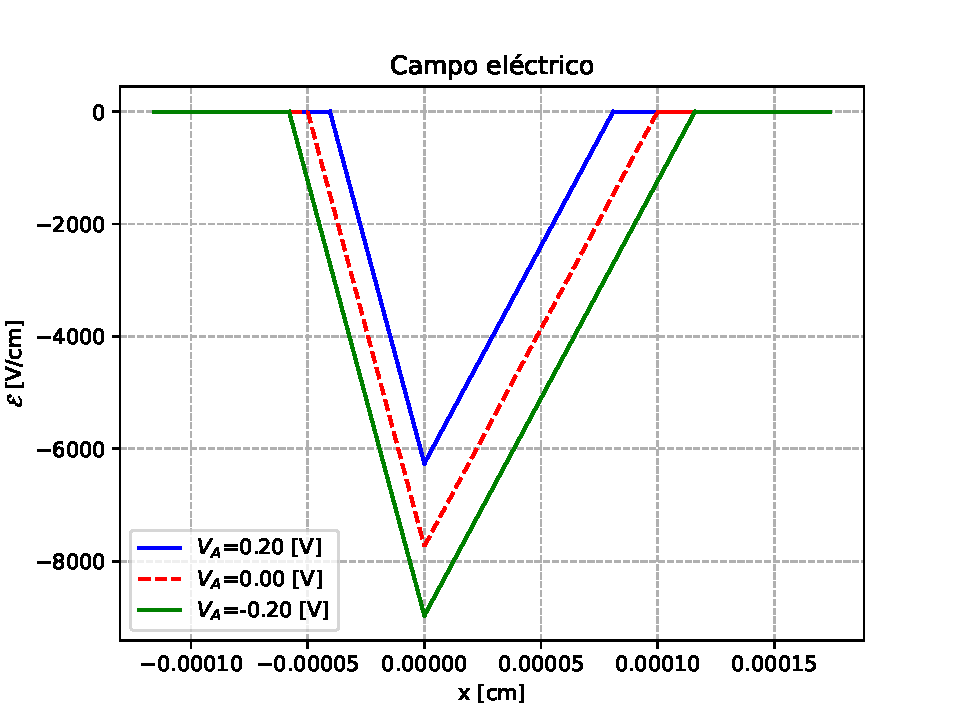
\includegraphics[width=\textwidth]{Ejercicios/Ch_03/03_04_E.pdf}
    \end{subfigure}
    \begin{subfigure}{0.47\textwidth}
        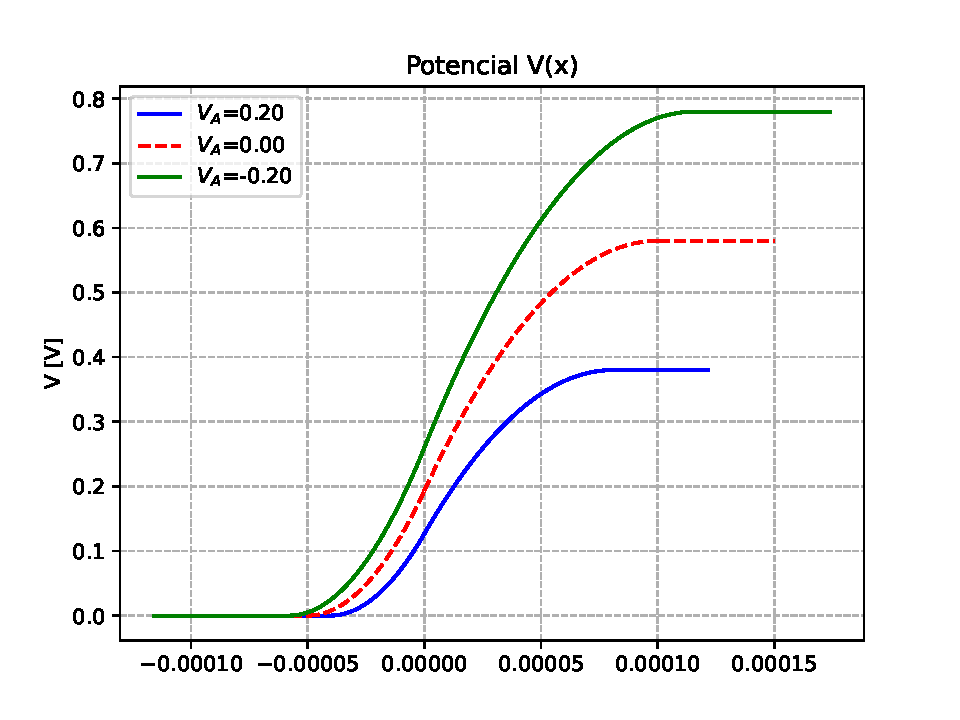
\includegraphics[width=\textwidth]{Ejercicios/Ch_03/03_05_V.pdf}
    \end{subfigure}
    \end{figure}
    \begin{center}
        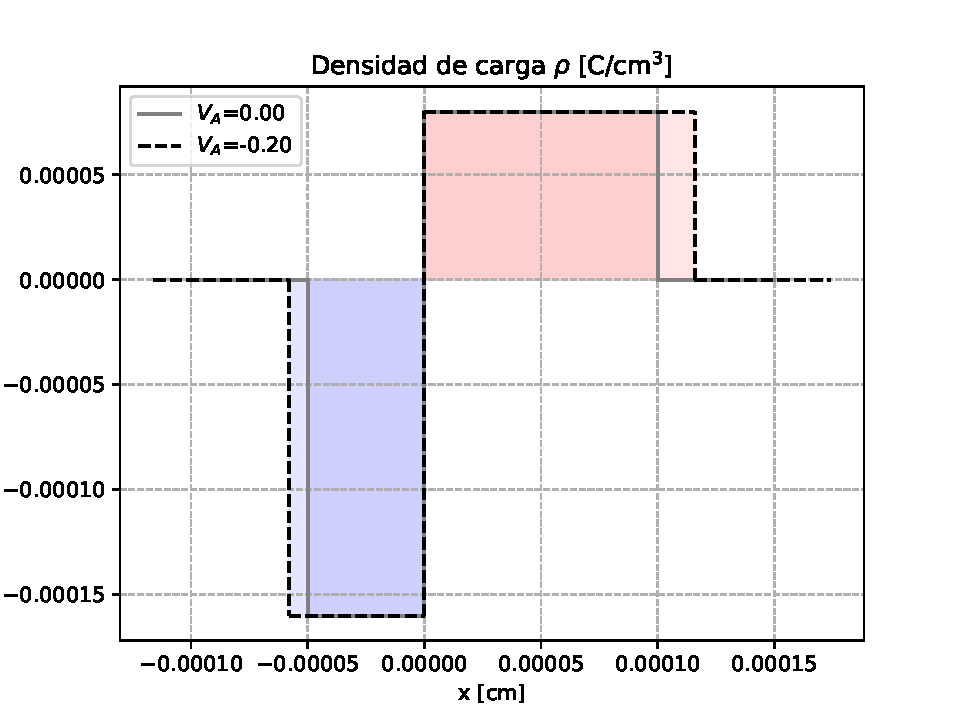
\includegraphics[width=0.6\linewidth]{Ejercicios/Ch_03/03_06_rho.pdf}
    \end{center}   
    Ahora tenemos que calcular las corrientes a lo largo del dispostivo. Las corrientes de cada portador dependen (al menos la forma funcional) depende principalmente de si nos encontramos en la región maiva $N/P$ o en la región de vaciamiento. 
    Los valroes más relevantes son aquellos que se dan en $x_n$ y $x_p$, ya que definen los valores tanto en la zona masiva como los valores en la zona de vaciamiento. Así pues, tenemos:

    \begin{equation}
        I_N (-x_p) = \frac{AqD_N}{L_N}  \frac{n_i^2}{N_A} \parentesis{e^{qV_A/kT}-1} \qquad
        I_P (x_n) = \frac{AqD_P}{L_P} \frac{n_i^2}{N_D}  \parentesis{e^{qV_A/kT}-1}
    \end{equation}
    que numéricamente se expresa como:
    \begin{equation}
        I_N (-x_p) = -8.55\cdot10^{-13} \ [\unit{A}] \qquad 
        I_P (x_n) = -9.95 \cdot 10^{-13}\ [\unit{A}]
    \end{equation}
    donde hemos usado que:

    \begin{equation}
        D_N = 35.1 \ [\unit{cm^2/s}] \quad 
        D_P = 11.9 \ [\unit{cm^2/s}] \quad L_N = 5.92 \cdot 10^{-3} \ [\cm] \end{equation}
    \begin{equation}     
        L_P = 3.45 \cdot 10^{-3} \ [\cm]  \quad n_i = 9.49 \cdot 10^{9} \ [\cm^{-3}]
    \end{equation}
    Veamos que la corriente total es:    

    \begin{equation}
        I = I_0 \parentesis{e^{qV_A/kT}-1} = I_N (-x_p) + I_P (x_n) \qquad  I_0 =  A q \parentesis{\frac{D_N}{L_N} n_{p0} + \frac{D_P}{L_P} p_{n0}}
    \end{equation}
    Con un resultado numérico de: 

    \begin{equation}
        I =  18.5 \cdot 10^{-13} \ [\unit{A}]
    \end{equation}
    Al tener un $L_N$ y $L_P$ bastante alto (de hecho del orden del tamaño del diodo) es normal que la representación gráfica sea bastante mala, y que no seamos capaces de ver esa tendencia a cero y a $I_T$ de $I_N$ e $I_P$. Usando las ecuaciones del diodo estrecho obtenemos los siguientes valores numéricos: 

    \begin{equation}
        I_N(x_p)=\SI{-9.804e-13}{[A]} \qquad  
        I_P(x_n)=\SI{-1.015e-12}{[A]} 
    \end{equation}
    \begin{equation}
        I = \SI{-1.995e-12}{[A]}
    \end{equation}
    Con la siguiente representación gráfica:
    \begin{center}
    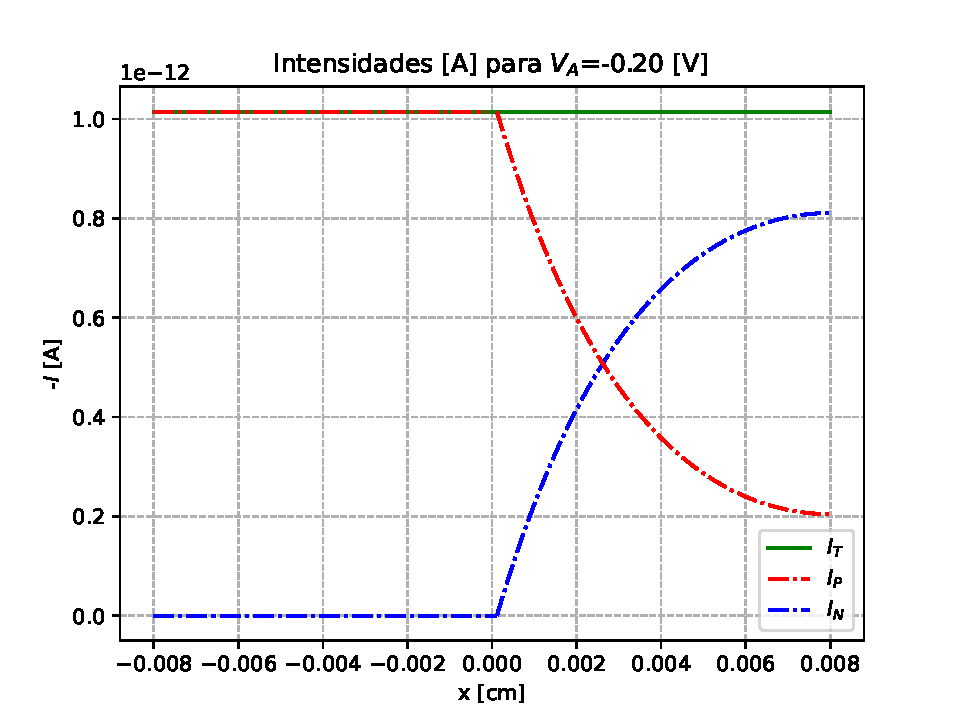
\includegraphics[width=0.6\linewidth]{Ejercicios/Ch_03/03_07_I.pdf}
    \end{center}

\end{enumerate}    
%%%%%%%%%%%%%%%%%%%%%%%%%%%%%%%%%%%%%%%%%%%%%%%%%%%%%%%%%%%%%%%%%%%%%%%
%%%%%%%%%%%%%%%%%%%%%%%%% EJERCICIOS 2 %%%%%%%%%%%%%%%%%%%%%%%%%%%%%%%%
%%%%%%%%%%%%%%%%%%%%%%%%%%%%%%%%%%%%%%%%%%%%%%%%%%%%%%%%%%%%%%%%%%%%%%%

\begin{Enunciado}
\subsection*{Ejercicios 2}

Partimos de una unión escalón NP realizada con un cristal semicondcutor de germanio ($E_G = 0.66 \ \eV$, $m_e^*=0.5$, $m_h^* = 0.37$) con $N_D=10^{16} \ \cm^{-3}$ y $N_A = 10^{15} \ \cm^{-3}$, en cada zona siendo la longitud de la zona $N$ de 0.003 cm y la de la zona P de 0.002 cm y el área de $10^{-2} \ \cm^2$. La permitividad para el germanio es de $1.4337 \times 10^{-12}$ F/cm, y el $n_i=2.0 \times 10^{13}$ cm$^{-3}$, las movilidades de electrones y huecos son $3900$ cm$^2$/(V$\cdot$s) y $1900$ cm$^2$/(V$\cdot$s) respectivamente y $\tau_n=\tau_p=10^{-6}$ s.

\begin{enumerate}[label=\alph*)]
    \item Para la situación de equilibrio, comprobar que no esté degenerado y calcular el potencial de contacto, el ancho de la región de vaciamiento y el campo eléctrico máximo.
    \item Calcula los incrementos de los portadores minoritarios en los bordes de las zonas de vaciamiento para los voltajes -0.1 y 0.1. Representa gráficamente la distribución de los portadores minoritarios e indica razonadamente si se podría aplicar la hipótesis de bajo nivel de inyección para esas polarizaciones.
    \item Calcula la corriete total y las componentes de corriente de electrones y huecos en la zona de vaciamiento para esas polarizaciones. Indica además la relación entre ellas. Representa gráficametne como varían las corrientes de electrones y huecos a lo largo de todo el dispositivo. 
\end{enumerate}
\end{Enunciado}


\begin{enumerate}[label=\alph*)]
    \item Para la situación de equilibrio comprobar que no está degenerado es sencillo, aunque necesitamos conocer la temeratura. La temperatura que tiene que haber para que nuestro gap sea $E_g=0.66\eV$ es de aproximadamente $\sim 310$K. ¿Cómo sabemos esto? Pues aplicando la ecuación de Varshini pero a la inversa. Nosotros usaremos $300$K ya que es la temperatura que usamos en todos los ejercicios, y tampoco dista mucho de la temperatura real. Así pues, para 300K, veamos que no está degenerado ya que en la gráfica: 
    \begin{center}
        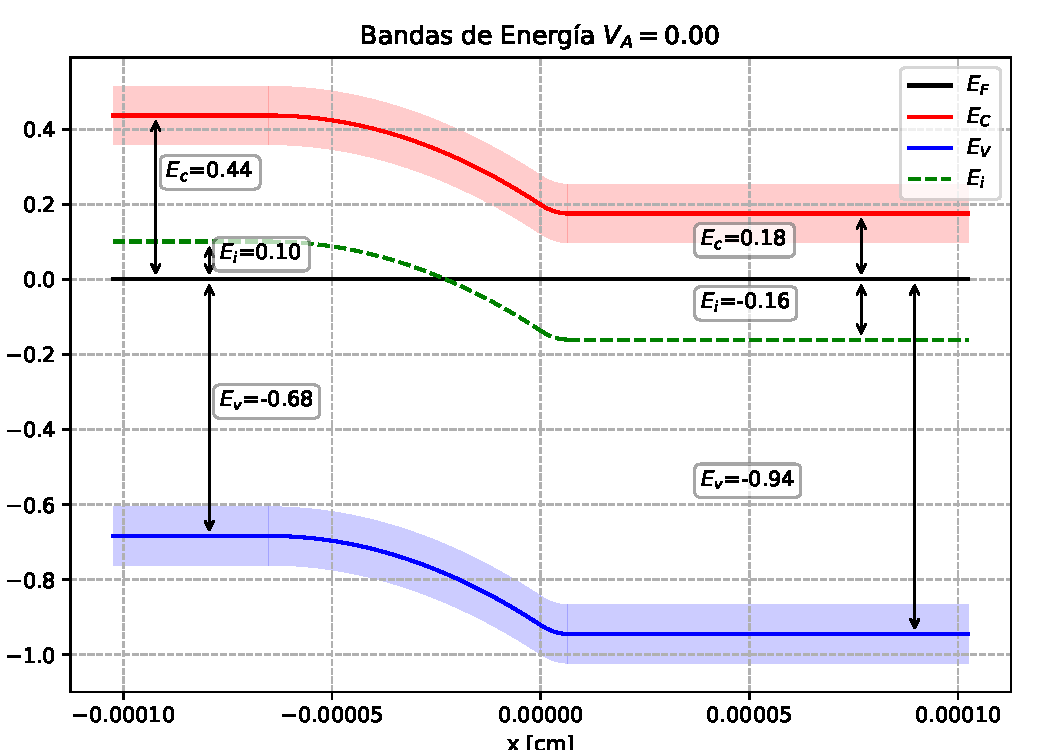
\includegraphics[width=0.6\linewidth]{Ejercicios/Ch_03/03_08_Bandas.pdf}
    \end{center}
    tal que $3k_B\cdot 300=0.078 \ \eV$. Estamos lejos de que esté degenerado. Así pues: 

    \begin{equation}
        \Vbi = 0.26 \eV \qquad x_p=6.51871 \cdot 10^{-5} \ [cm] \qquad 
        x_n= 6.51871 \cdot 10^{-6} \ [cm]
    \end{equation}
    El campo eléctrico máximo por otro lado: 

    \begin{equation}
        \Ecal_{\max}=-7284.73 \ [\unit{V/cm}]
    \end{equation}
    que se deduce de la ecuación 
    \begin{equation}
        \Ecal = - \frac{qN_A}{K_S\varepsilon_0} x_p = - \frac{qN_D}{K_S\varepsilon_0} x_n
    \end{equation}
    \item  Los incrementos de portadores minoritarios en los bordes de las zonas viene dado por:
    \begin{equation}
        \Delta n = \frac{n_i^2}{N_A} \parentesis{e^{qV_A/kT}-1}  \tquad 
        \Delta p = \frac{n_i^2}{ND} \parentesis{e^{qV_A/kT}-1} 
    \end{equation}
    Así pues, los valores numéricos son:

    \begin{equation}
        V_A=0.1 \ [\unit{V}] \qquad  \Delta n = \ [\cm^{-3}] \quad \Delta p = \ [\cm^{-3}]
    \end{equation}
    \begin{equation}
        V_A=-0.1 \ [\unit{V}] \qquad  \Delta n = \ [\cm^{-3}] \quad \Delta p = \ [\cm^{-3}]
    \end{equation}
    Calculamos $L_N$ y $L_P$ para comprobar si tenemos que usar las ecuaciones del diodo estrecho:

    \begin{equation}
        D_N =100.1 \ [\unit{cm^2/s}] \quad 
        D_P=\SI{4.92e+01}{}\ [\unit{cm^2/s}] 
    \end{equation}
    \begin{equation}    
        L_N=\SI{1.00e-02}{} \ [\unit{cm}] \quad
        L_P=\SI{7.01e-03}{} \ [\unit{cm}]
    \end{equation}
    Como podemos ver, el tamaño del diodo es del tamaño de $L_N,L_P$. Consecuentemente tenemos que usar las ecuaciones del diodo estrecho. Tenemos que: 
   \begin{equation}
    V_A=0.1: \qquad x_p=5.12090e-05 [cm] \quad  
    x_n=5.12090e-06 [cm]
   \end{equation}
   \begin{equation}
    V_A=-0.1: \qquad 
    x_p=\SI{7.66573e-05 }{[cm]} \quad 
    x_n=\SI{7.66573e-06}{[cm]}
   \end{equation}
   Como podemos ver en la siguiente imagen, la aproximación a baja inyección es suficientemente buena:
   \begin{center}
    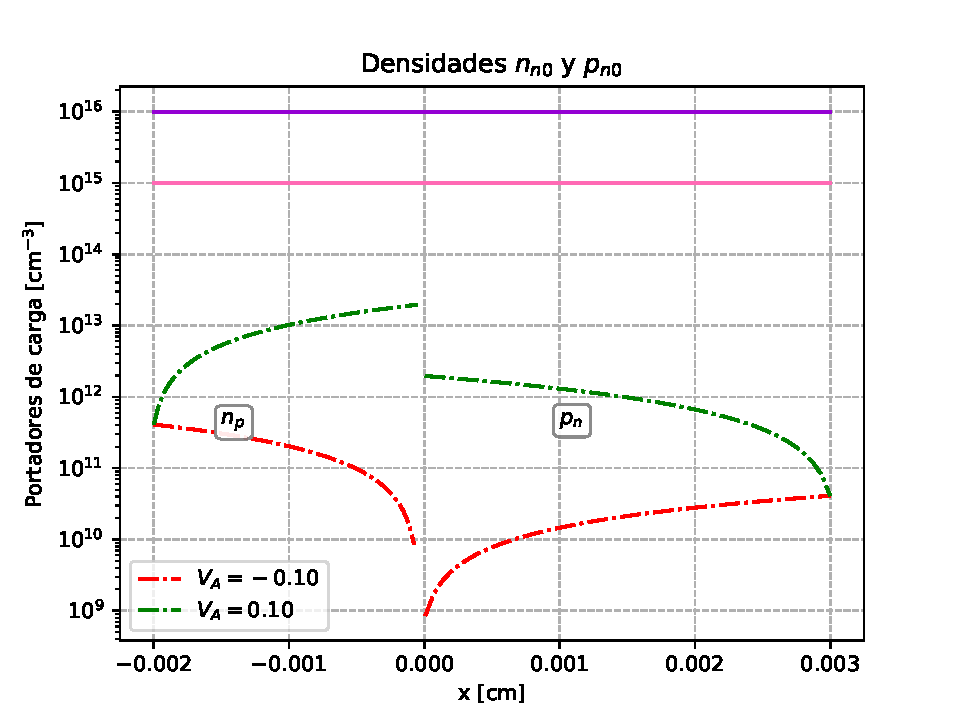
\includegraphics[width=0.7\linewidth]{Ejercicios/Ch_03/03_09_portadores.pdf}
   \end{center}
    \item Calculamos la corriente total y las componentes en la siguiente imagen (usando las ecuaciones del diodo estrecho):
    \begin{equation}
        I_{P}(x_n) = q A \frac{D_P}{L_P} p_{n0} \coth \parentesis{\frac{x_{1n}-x_n}{L_N}}  \parentesis{e^{qV_A/kT}-1} 
    \end{equation}
    \begin{equation}
        I_{N}(x_p) = q A \frac{D_N}{L_N} n_{p0} \coth \parentesis{\frac{x_{1p}-x_p}{L_N}}  \parentesis{e^{qV_A/kT}-1}
    \end{equation}
    Tal que los resultados numéricos son: 
    \begin{equation}
        V_a=\SI{1.0e-01}{[V]} \quad 
        I_N(x_p)=\SI{1.610e-03}{[A]} \quad 
        I_P(x_n)=\SI{5.346e-05}{[A]}
    \end{equation}
    \begin{equation}
        I_T = \SI{1.663e-03}{[A]}
    \end{equation}
    \begin{equation}        
        V_a=\SI{-1.0e-01}{[V]} \quad 
        I_N(x_p)=\SI{-3.409e-05}{[A]} \quad 
        I_P(x_n)=\SI{-1.118e-06}{[A]}
    \end{equation}
    \begin{equation}
        I_T = \SI{-3.52e-05}{[A]}
    \end{equation}
    \begin{center}
     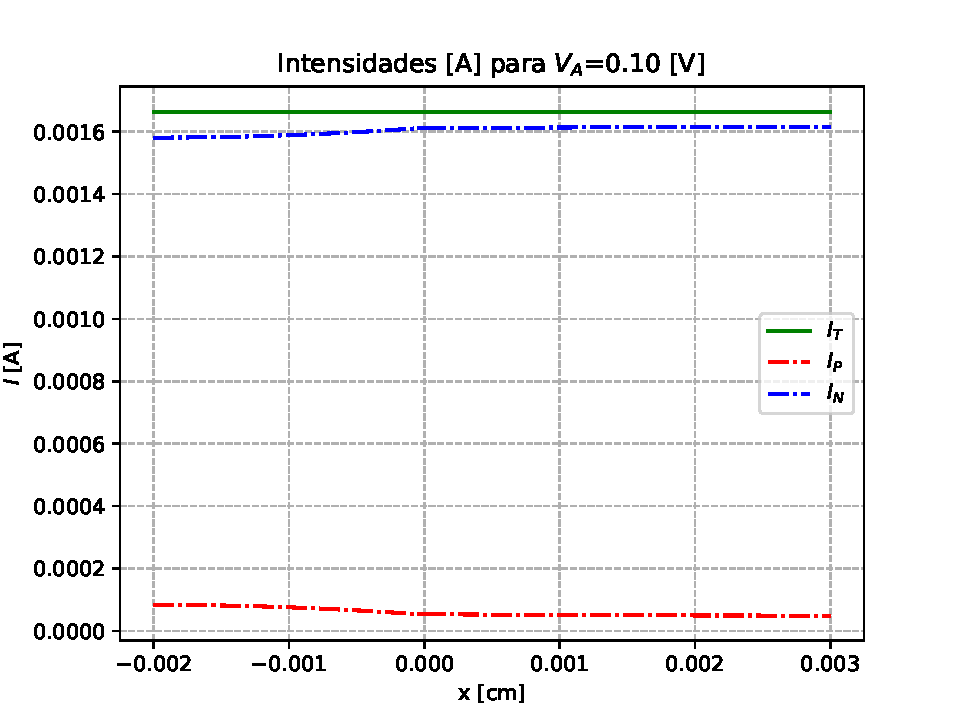
\includegraphics[width=0.7\linewidth]{Ejercicios/Ch_03/03_10_corrientes.pdf}
    \end{center}
    \begin{center}
     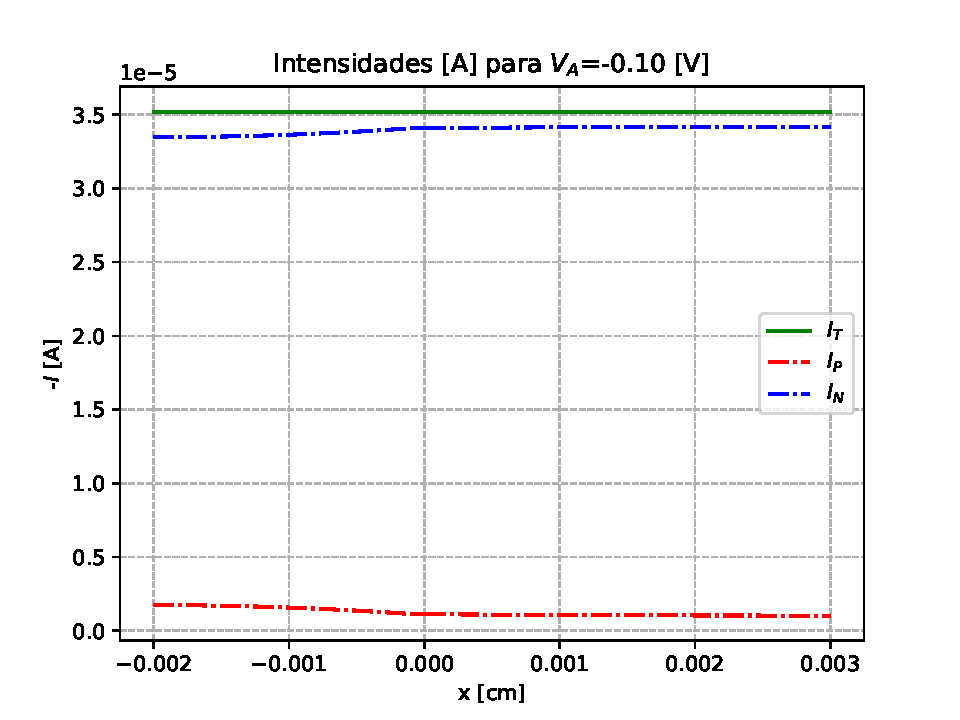
\includegraphics[width=0.7\linewidth]{Ejercicios/Ch_03/03_11_corrientes.pdf}
    \end{center}
    
\end{enumerate}



%---------------------------
% Ejercicio 3
%---------------------------

\begin{Enunciado}
	\subsection*{Ejercicio 3}
	%\addcontentsline{toc}{subsection}{\textit{Ejercicio 3}}
    
	\lipsum[1].
\end{Enunciado}

\vspace*{1em}

\lipsum[1].

%---------------------------
% Ejercicio 4
%---------------------------

\begin{Enunciado}
	\subsection*{Ejercicio 4}
	%\addcontentsline{toc}{subsection}{\textit{Ejercicio 4}}
    
	\lipsum[1].
\end{Enunciado}

\vspace*{1em}

\lipsum[1].

\vspace*{2em}

%%%%%%%%%%%%%%%%%%%%%%%%%%%%%%%%%%%%%%%%%%%%%%%%%%%%%%%%%%%%%%%%%%%%%%%
%%%%%%%%%%%%%%%%%%%%%%%%% EJERCICIOS 5 %%%%%%%%%%%%%%%%%%%%%%%%%%%%%%%%
%%%%%%%%%%%%%%%%%%%%%%%%%%%%%%%%%%%%%%%%%%%%%%%%%%%%%%%%%%%%%%%%%%%%%%%


\subsection*{Ejercicio 5} 

\begin{Enunciado}
    
En una unión PN de silicio que en la zona de vaciamiento tiene $J_n = 25$ mA/cm$^2$ y 
$J_p = 7$ mA/cm$^2$ a $V_A = 0.5$ V. ($D_n = 21$ cm$^2$/s, $D_p = 10$ cm$^2$/s, 
$\tau_{p0} = \tau_{n0} = 5 \times 10^{-7}$ s), calcula y representa:

\begin{itemize}
    \item El diagrama de bandas de energía para esa polarización.
    \item La concentración de portadores de cada tipo en todo el dispositivo.
\end{itemize}


\end{Enunciado}
El ejercicio 5:

\begin{itemize}
    \item Nos dan los valores de $J_N$ y $J_P$ en la región de vaciamiento, cque vienen dadas por
    \begin{equation*}
        J_N = q \frac{D_N}{L_N} n_{p0} \parentesis{e^{qV_A/kT}-1}      \tquad    J_P = q \frac{D_P}{L_P} p_{n0} \parentesis{e^{qV_A/kT}-1}
    \end{equation*}
    y como conocemos $D_N,D_P,L_N,L_P$ y $V_A$, podemos despejar:
    \begin{equation}
        L_N = \sqrt{D_N \tau_n} = 0.32 \ \unit{cm} \qquad L_P = \sqrt{D_P \tau_p } = 0.22 \ \unit{cm}
    \end{equation}
    \begin{equation*}
        n_{p0} = \frac{J_N}{q} \frac{L_N}{D_N} \frac{1}{\parentesis{e^{qV_A/kT}-1} } = 9.6\cdot 10^5 \cm^{-3} \qquad p_{n0} = \frac{J_P}{q} \frac{L_P}{D_P} \frac{1}{\parentesis{e^{qV_A/kT}-1} }     = 3.9\cdot 10^5 \cm^{-3} 
    \end{equation*}
    Que como conocemos $n_i$ a la temperatura de 300 K:
    
    \begin{equation*}
        n_i = 10^{10} \ (\cm^{-3})
    \end{equation*}
    significa que podemos conocer $N_A$ y $N_D$, tal que:

    \begin{equation*}
        N_A = \frac{n_i^2}{n_{p0}} = \SI{1.042e+15}{cm^{-3}} \tquad N_D = \frac{n_i^2}{p_{n0}} = \SI{2.569e+15}{cm^{-3}} 
    \end{equation*}
    y ahora podemos usar las siguientes ecuaciones para calcular los valores de $E_c,E_i$ y $E_v$ respecto $E_F$: 

    \begin{equation*}
        E_i |_P =  kT \ln \parentesis{\frac{N_A}{n_i}} \quad E_c |_P = \frac{E_g}{2} + E_i + \frac{3}{4}kT \frac{m_n^*}{m_p^*} \quad E_v|_P = E_c|_P - E_g
    \end{equation*}
    Tal que:

    \begin{equation*}
        E_i|_N = E_i|_P - V_{bi} +V_a  \quad E_i|_N = E_i|_P - V_{bi} + V_a \quad E_i|_N = E_i|_P - V_{bi} +V_a
    \end{equation*}
    donde 
    \begin{equation*}
        \Vbi = \frac{kT}{q} \ln \parentesis{\frac{N_A N_D}{n_i^2}}  = 0.621 \ \unit{V}
    \end{equation*}       
    y así $\Vbi^\text{eff} = \Vbi - V_A = 0.121$ V. Falta escribir:
    
    \begin{equation}
        x_n = 1.32 \cdot 10^{-5} \ \cm \tquad x_p = 3.26 \cdot 10^{-5} \ \cm
    \end{equation}    
    El diagrama de bandas con polarización $V_A=0.5$ V

    \begin{center} 
        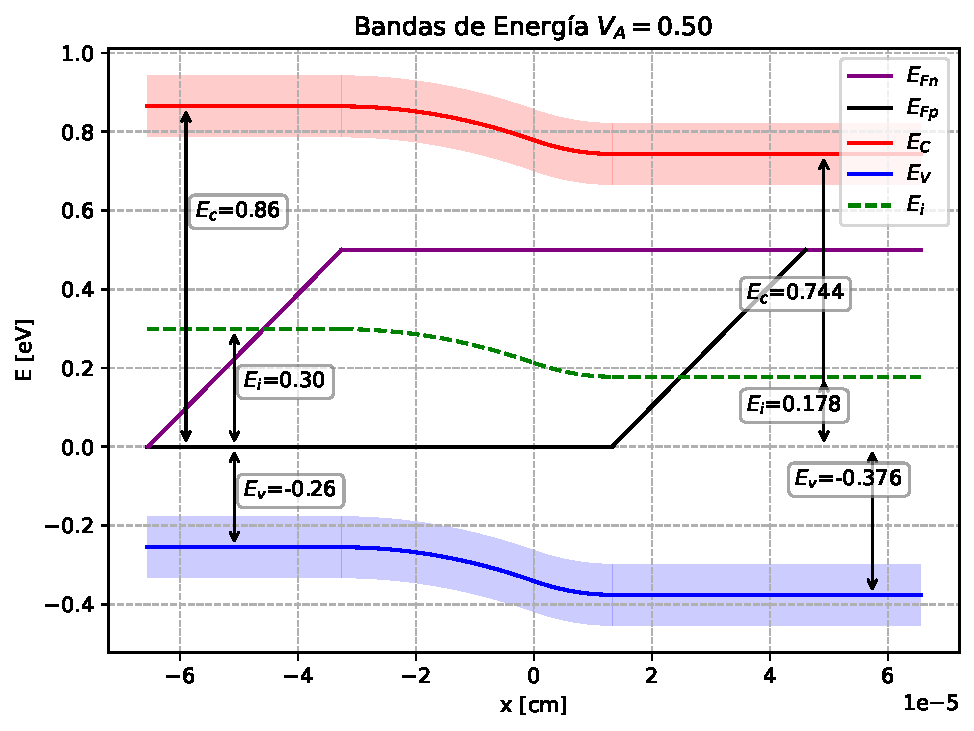
\includegraphics[width=0.7\linewidth]{Ejercicios/Ch_03/03_05_01.pdf}
    \end{center}


    \item La concentración de portadores en todo el dispositvo se calcula usando las siguientes ecuaciones, suponiendo un diodo ideal infinito: 
    
    \begin{equation*}
        n_{p} = n_{p0} + n_{p0} \parentesis{e^{qV_A/kT}-1} e^{(x+x_p)/kT}  \tquad  n_n = N_D
    \end{equation*}
    \begin{equation*}
        p_{p} = N_A \tquad p_{n} (x) = p_{n0} \parentesis{e^{qV_A/kT}-1} e^{-(x-x_n)/kT}  
    \end{equation*}
    En la región de vaciamiento suponemos que $n$ y $p$ son rectas que conectan los valores límites. La gráfica en el caso de polarización $V_A=0.5$ V: 
    \begin{figure}[h!] \centering
        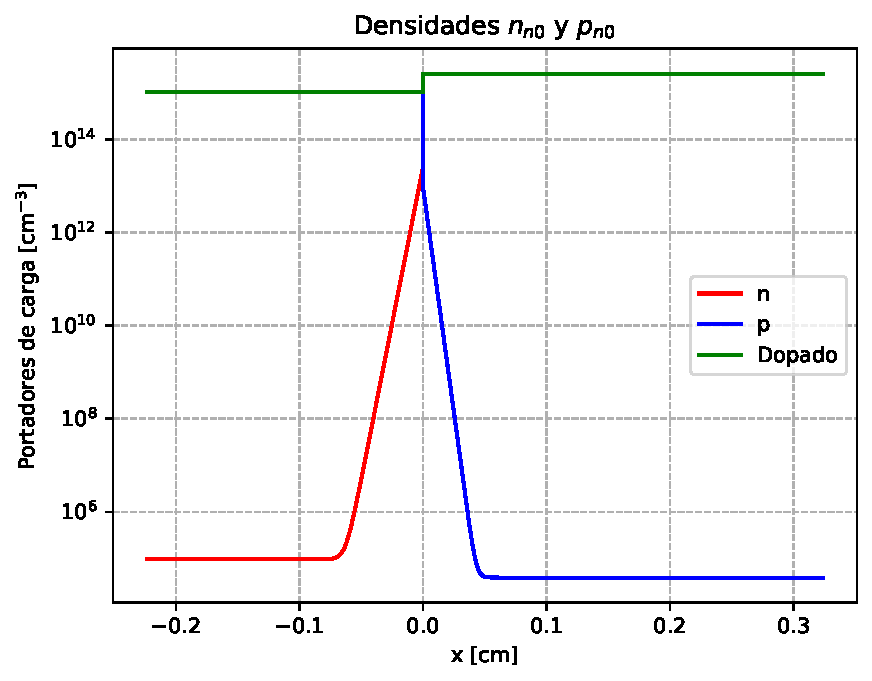
\includegraphics[width=0.7\linewidth]{Ejercicios/Ch_03/03_05_02.pdf}
    \end{figure}

\end{itemize}




%%%%%%%%%%%%%%%%%%%%%%%%%%%%%%%%%%%%%%%%%%%%%%%%%%%%%%%%%%%%%%%%%%%%%%%
%%%%%%%%%%%%%%%%%%%%%%%%% EJERCICIOS 6 %%%%%%%%%%%%%%%%%%%%%%%%%%%%%%%%
%%%%%%%%%%%%%%%%%%%%%%%%%%%%%%%%%%%%%%%%%%%%%%%%%%%%%%%%%%%%%%%%%%%%%%%

\subsection*{Ejercicio 6} 
\begin{Enunciado}
    

Si tenemos una unión NP polarizada en directa, $V_A = 0.2$ V:

\begin{itemize}
    \item Representar el diagrama de bandas de energía.
    \item Obtener el valor de la densidad de corriente de cada tipo de portador y representarla en todo el dispositivo.
\end{itemize}

Datos: $A = 2$ mm$^2$, $T = 300$ K, $E_{gap} = 1.42$ eV, $N_D = N_A = 10^{14}$ cm$^{-3}$, $\mu_n = 9000$ cm$^2$/Vs, $\mu_p = 450$ cm$^2$/Vs, $\tau_p = 20$ ns, $\tau_n = 10$ ns, $\varepsilon = 1.4337 \times 10^{-12}$ F/cm, $m_e/m_0 = 0.4$, $m_h/m_0 = 0.3$.


\end{Enunciado}

Hay que recordar que una unión np es igual que la union pn pero donde $x\rightarrow -x$
\begin{itemize}
    \item Usamos las siguientes ecuaciones para calcular los valores de $E_c,E_i$ y $E_v$ respecto $E_F$: 
    
    \begin{equation*}
        E_i|_P =  k T \ln \parentesis{\frac{N_A}{n_i}} \qquad E_c|_P = \frac{E_g}{2} + E_i + \frac{3}{4} kT \ln \parentesis{\frac{m_n^*}{m_p^*}} \qquad E_v |_P = E_c - E_g
    \end{equation*}
    \begin{equation*}
        E_i|_N = E_i - \Vbi^\text{eff}  \qquad E_c|_N = E_c|_N - \Vbi^\text{eff} E_v |_N = E_v|_N - \Vbi^\text{eff} 
    \end{equation*}
    donde hemos usado que ($K_S=16.2$)

    \begin{equation*}
        n_i = 2 \parentesis{\frac{kT (m_n^* m_p^* )^{1/2}}{2\pi \hbar^2}}^{3/2} e^{-\frac{E_g}{2kT}} 
    \qquad \Vbi^{\text{eff}} = \Vbi - V_a \quad \Vbi = \frac{kT}{q} \ln \parentesis{\frac{N_AN_D}{n_i^2}}
    \end{equation*}
    \begin{equation}
        n_i=\SI{6.046e+6}{cm^{-3}} \quad \Vbi = 0.859 
    \end{equation}
    \begin{equation}
        D_N = 232.67 \ \cm^2/s \quad D_P =  11.63 \ \cm^2/s \quad L_N = 15.21 \ \mu \unit{m} \quad L_P = 4.82 \  \mu \unit{m}
    \end{equation}
    \begin{equation}
        x_n = \SI{2.429e-4}{cm} \tquad 
        x_p = \SI{2.429e-4}{cm}  
    \end{equation}
    Así pues, el diagrama de bandas con polarización $V_A=0.5$ V: 

    \begin{center} 
        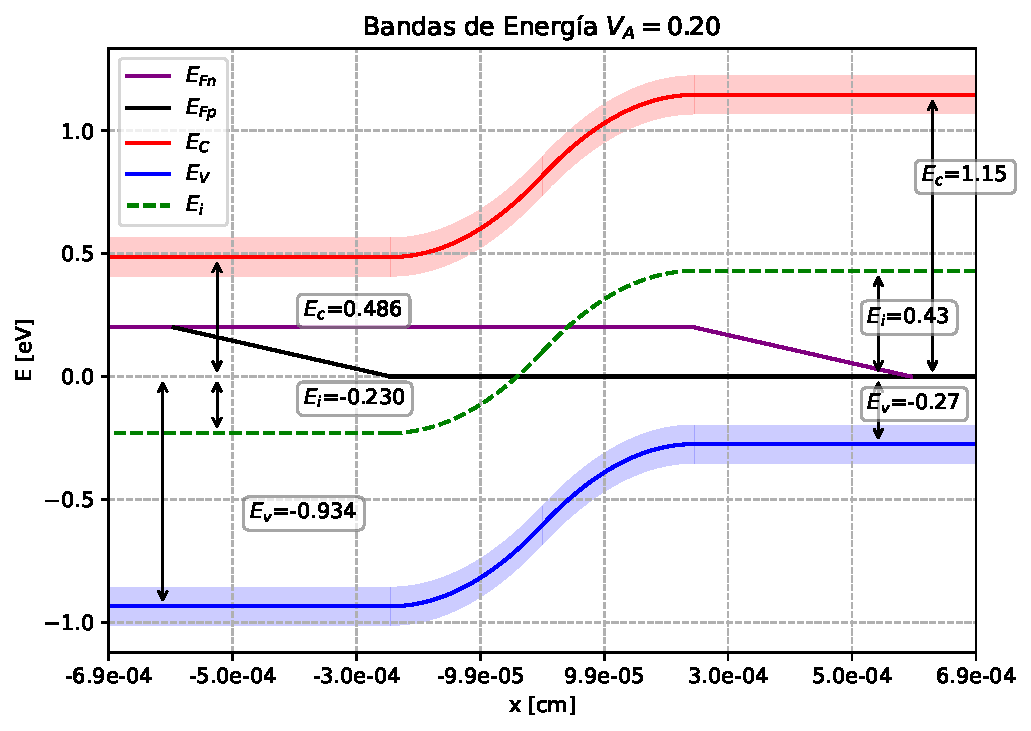
\includegraphics[width=0.6\linewidth]{Ejercicios/Ch_03/03_06_01.pdf}
    \end{center}
    

    \item Los valores de las intensidades en todo el dispositvo se calcula usando las siguientes ecuaciones: 
    
    \begin{equation*}
        \text{Zona P:} \quad 
        I_N(x) = -qA\frac{D_N}{L_N} \frac{n_i^2}{N_A}  \parentesis{e^{qV_A/kT}-1} e^{(x+x_p)/L_N} \quad I_P(x) = I_T - I_N (x)
    \end{equation*}
    \begin{equation*}
        \text{Zona N:} \quad 
        I_P(x) = - qA\frac{D_P}{L_P} \frac{n_i^2}{N_D}  \parentesis{e^{qV_A/kT}-1} e^{(-x+x_n)/L_P} \quad I_N(x) = I_T - I_P (x)
    \end{equation*}
    tal que:

    \begin{equation*}
        I_T = -qA\parentesis{\frac{D_N}{L_N} \frac{n_i^2}{N_A}+\frac{D_P}{L_P} \frac{n_i^2}{N_D}}  \parentesis{e^{q V_A/kT}-1}
    \end{equation*}
    Al ser NP tenemos que el signo cambia, al ser polarización directa la corriente va de P a N (recordemos que en polarización directa predomina la corriente de difusión, que tiene la dirección P$\rightarrow$M, que en este caso significa corriente negativa). Y los valores numéricos:

    \begin{equation}
        I_P (x_n) = \SI{-6.467e-14}{C/s} \qquad 
        I_N (x_p) = \SI{-4.737e-13}{C/s} \qquad
        I_T = \SI{4.737e-13}{C/s}
    \end{equation}

    Obteniendo la siguiente gráfica para $V_A=0.2$ V: 


    \begin{center} 
        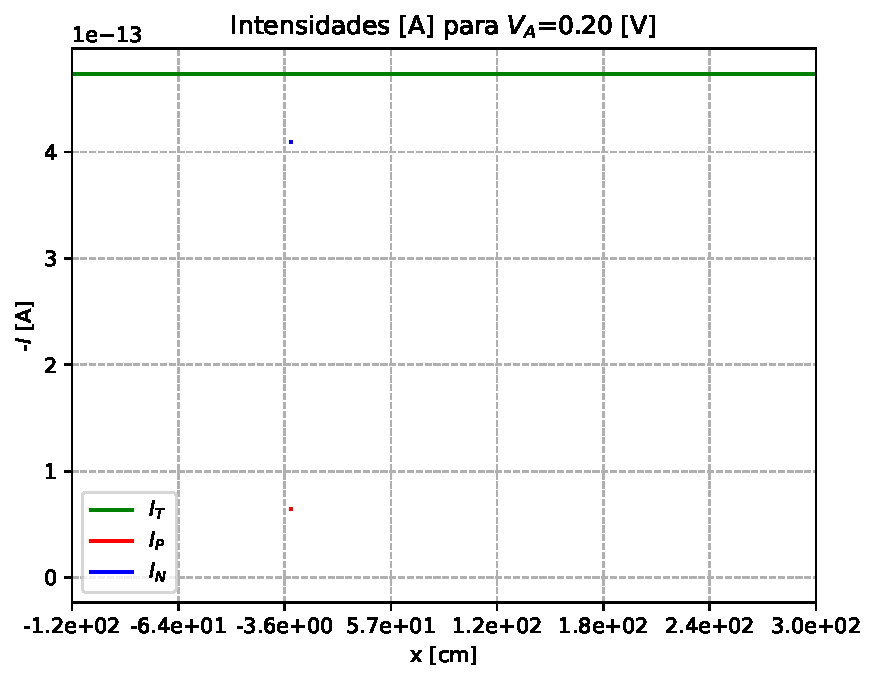
\includegraphics[width=0.6\linewidth]{Ejercicios/Ch_03/03_06_02.pdf}
    \end{center}
    
\end{itemize}



%%%%%%%%%%%%%%%%%%%%%%%%%%%%%%%%%%%%%%%%%%%%%%%%%%%%%%%%%%%%%%%%%%%%%%%
%%%%%%%%%%%%%%%%%%%%%%%%% EJERCICIOS 7 %%%%%%%%%%%%%%%%%%%%%%%%%%%%%%%%
%%%%%%%%%%%%%%%%%%%%%%%%%%%%%%%%%%%%%%%%%%%%%%%%%%%%%%%%%%%%%%%%%%%%%%%

\begin{Enunciado}
\subsection*{Ejercicio 7} 

Si partimos de una unión PN de silicio, con el lado P dopado de forma gradual con 
$a = 10^{19}$ cm$^{-4}$ y el lado $N_D = 3.0 \times 10^{14}$ cm$^{-3}$ constante. 
Bajo condición de equilibrio, si el ancho de la zona de vaciamiento de la zona P es 
de 0.8 micras, calcular y representar el ancho total de la zona de vaciamiento, 
el campo eléctrico y el potencial de contacto.

\end{Enunciado}

Si suponemos que la densidad de carga es:

\begin{equation*}
    \rho (x) = \left\lbrace \begin{array}{ll}
        -q a x & -x_p < x < 0  \\ 
        q N_D & 0 < x < x_n  
    \end{array} \right.
\end{equation*}
El campo eléctrico viene dado por:

\begin{equation*}
    \Ecal (x) =  \left\lbrace \begin{array}{ll}
        \frac{qa}{2K_S\varepsilon_0} \ccorchetes{x^2 - x_p^2} & -x_p < x < 0  \\ 
        \frac{qN_D}{K_S\varepsilon_0} \ccorchetes{x- x_n} & 0 < x < x_n  
    \end{array} \right. 
\end{equation*}
\begin{equation*}
    \Ecal_{\min} = -49500 \ \unit{V/cm} 
\end{equation*}
Exigimos que el campo en $x=0$ debe ser igual en ambos lados:

\begin{equation}
    \frac{qN_D}{K_S \epsilon_0} x_n = \frac{qa}{2K_S\epsilon_0} x_p^2 \rightarrow x_n = \frac{a x_p^2}{2 N_D} = 1.06 \ \unit{\mu m} \quad W = 1.86 \ \unit{\mu m}
\end{equation}


donde hemos exigido que $\Ecal(x_n)=0$ y $\Ecal(-x_p)=0$. El potencial de contacto:
\begin{equation*}
    V (x) =  \left\lbrace \begin{array}{ll}
        \frac{qa}{6K_S\varepsilon_0} \ccorchetes{x^3 - 3x_p^2 x + A} & -x_p < x < 0  \\ 
        \frac{qN_D}{2K_S\varepsilon_0} \ccorchetes{x^2 - 2x_n x + B} & 0 < x < x_n  
    \end{array} \right.
\end{equation*} 
Para que $V(-x_p)=0$ tendría que verificarse $A=2x_p^3$. También se tiene que verficiar que $V(0)|_{-}=V(0)|_{+}$, y por tanto: 

\begin{equation*}
    \frac{qa A}{6K_S\varepsilon_0} = \frac{qN_D B}{2K_S\varepsilon_0} \rightarrow B = \frac{2 a x_p^3}{3 N_D}
\end{equation*}
El valor del voltaje final: 
\begin{equation*}
    V (x) =  \left\lbrace \begin{array}{ll}
        \frac{qa}{6K_S\varepsilon_0} \ccorchetes{-x^3 + 3x_p^2 x + 2x_p^3} & -x_p < x < 0  \\ 
        \frac{qN_D}{2K_S\varepsilon_0} \ccorchetes{-x^2 + 2x_n x + \frac{2 a x_p^3}{3 N_D}} & 0 < x < x_n  
    \end{array} \right.
\end{equation*}
Sería interesante definir ahora el valor de $\Vbi$ y vr si coincide con $V(x_n)$. Así tenemos que:

\begin{equation}
    \Vbi = \frac{qN_D}{2K_S\epsilon_0} \ccorchetes{-x_n+\frac{2ax_p^3}{3N_D}} = 0.525 \ \unit{V}
\end{equation}
Tenemos pues que: 
\begin{equation}
    \Vbi^* = \frac{kT}{q} \ln \parentesis{\frac{x_p a N_D}{n_i^2}} = 0.558 \ \unit{V}
\end{equation}



%---------------------------
% Ejercicio 7
%---------------------------
\begin{Enunciado}
	\subsection*{Ejercicio 8}
	%\addcontentsline{toc}{subsection}{\textit{Ejercicio 7}}
	\lipsum[1].
\end{Enunciado}
\vspace*{1em}
\lipsum[1].
\vspace*{2em}

%---------------------------
% Ejercicio 8
%---------------------------
\begin{Enunciado}
	\subsection*{Ejercicio 9}
	%\addcontentsline{toc}{subsection}{\textit{Ejercicio 8}}
    
	\lipsum[1].
\end{Enunciado}
\vspace*{1em}
\lipsum[1].
\vspace*{2em}
%---------------------------
% Ejercicio 9
%---------------------------
\begin{Enunciado}
	\subsection*{Ejercicio 10}
	%\addcontentsline{toc}{subsection}{\textit{Ejercicio 9}}
    
	\lipsum[1].
\end{Enunciado}
\vspace*{1em}
\lipsum[1].
